\section{Технологический раздел }

В соответствии с поставленной задачей, проект должен быть доступен пользователю быстро и не требовать сложной установки.

В настоящее время все больше проектов используют браузер для отображения пользовательского интерфейса.

\subsection{Стек технологий}

Данное приложение разрабатывалось на основе Django, фреймворка для веб-приложений на языке Python. Фреймворк использует схему разделения данных MVC. Данный шаблон проектирования используется для разделения приложения, логики и пользовательского интерфейса, что позволяет модифицировать их отдельно друг от друга.
\\

MVС состоит из трех компонентов: модели (Model), представления (View) и контроллера (Controller).  

\begin{figure}[H]
\center{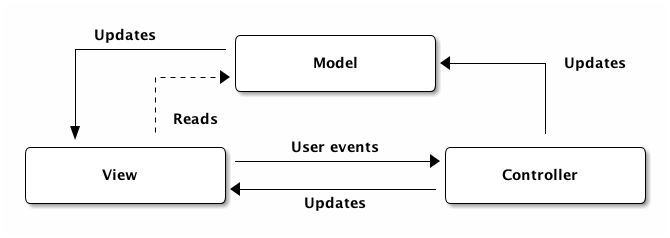
\includegraphics[width = 1\linewidth]{mvc}}
\caption{Паттерн MVC}
\end{figure}

Модель описывает используемые в приложении данные и реагирует на команды контроллера. Представление отвечает за отображение данных модели пользователю, реагируя на изменения модели. Контроллер обрабатывает действия пользователя и взаимодействует с моделью.
\pagebreak

\subsection{Взаимодействие с ПО}



\pagebreak
